% PACKAGES
\documentclass[a4paper, hidelinks, 12pt]{report}
\usepackage[margin=1in]{geometry}
\usepackage{amsfonts,amsmath,amssymb}
\usepackage[none]{hyphenat}
\usepackage{fancyhdr}
\usepackage{graphicx}
\usepackage{float}
\usepackage[nottoc,notlot,notlof]{tocbibind}
\usepackage{hyperref}
\usepackage{longtable}
\usepackage[utf8]{inputenc}
\usepackage{booktabs}
\usepackage{multirow}
\usepackage{booktabs}
\usepackage[font=footnotesize]{caption}
\usepackage[flushleft]{threeparttable}
\usepackage{amsmath}
\usepackage{relsize}
\usepackage[super,negative]{nth}
\usepackage{enumerate}
\usepackage{float}
\usepackage{rotating}
\usepackage[dvipsnames]{xcolor}
\usepackage{listings}
%%%%%%%%%%%%

% DOC STYLES
\makeatletter
\def\thickhrulefill{\leavevmode \leaders \hrule height 1ex \hfill \kern \z@}
\def\@makechapterhead#1{
	\vspace*{4\p@}
	{\parindent \z@ \centering \reset@font
		\thickhrulefill\quad
		\scshape \@chapapp{} \thechapter
		\quad \thickhrulefill
		\par\nobreak
		\vspace*{4\p@}
		\interlinepenalty\@M
		\hrule
		\vspace*{4\p@}
		\Huge \bfseries #1\par\nobreak
		\par
		\vspace*{4\p@}
		\hrule
		\vskip 50\p@
}}
\def\@makeschapterhead#1{
	\vspace*{4\p@}
	{\parindent \z@ \centering \reset@font
		\thickhrulefill
		\par\nobreak
		\vspace*{4\p@}
		\interlinepenalty\@M
		\hrule
		\vspace*{4\p@}
		\Huge \bfseries #1\par\nobreak
		\par
		\vspace*{4\p@}
		\hrule
		\vskip 50\p@
}}

\pagestyle{fancy}
\fancyhead{}
\fancyfoot{}
\fancyhead[L]{\slshape\MakeUppercase{\textbf{DD}}}
\fancyhead[R]{\slshape{Avila, Schiatti, Virdi}}
\fancyfoot[C]{\thepage}
\renewcommand{\footrulewidth}{1pt}
\renewcommand{\headrulewidth}{1pt}
\linespread{1.3}
%\floatstyle{boxed}
\restylefloat{figure}
\parindent 0ex
%\renewcommand{baselinestretch}{1.5}

%%%%%%%%%%%%

% COMMANDS
\newcommand\requirement[1]{\item[{[R#1]}] }
\newcommand\goal[1]{\item[{[G#1]}] }
\newcommand\assumption[1]{\item[{[D#1]}] }
\newcommand\usecase[1]{ [UC#1] }

%%%%%%%%%%%%

%BODY
\begin{document}
	\begin{titlepage}
		\centering
		\vspace*{0.7 cm}
		\includegraphics[scale = 0.85]{../Assets/PolimiLogo.png}\\[1.6 cm]
		\textsc{\large Department of Computer Science and Engineering}\\[1.8 cm]
		
		\rule{\linewidth}{0.2 mm} \\[0.4 cm]
		{ \huge \bfseries Design Document (DD)}\\
		\rule{\linewidth}{0.2 mm} \\[1.5 cm]
		
		\textsc{\Large TrackMe}\\[0.5 cm]
		\textsc{\large - v1.0 -}\\[1 cm]
		
		\begin{minipage}{0.4\textwidth}
			\begin{flushleft} \large
				\emph{Authors:}\\
				\textbf{Avila}, Diego \\
				\textbf{Schiatti}, Laura \\
				\textbf{Virdi}, Sukhpreet
			\end{flushleft}
		\end{minipage}~
		\begin{minipage}{0.4\textwidth}
			\begin{flushright} \large
				%\emph{Student Number:} \\
				903988 \\
				904738 \\
				904204
			\end{flushright}
		\end{minipage}\\[2 cm]
		
		{\large December \nth{10} , 2018}\\[2 cm]
		
		\vfill
	\end{titlepage}
	
	\pagenumbering{roman}
	\tableofcontents
%	\thispagestyle{empty}
	\newpage
	\listoffigures
	\listoftables
%	\thispagestyle{empty}
	\clearpage
	\pagenumbering{arabic}
	\setcounter{page}{1}
	
	\chapter{Introduction}
	\section{Context}
	\textbf{TrackMe} develops health-monitoring devices devoted to measure and record different parameters related to the health status of a person (i.e. body temperature, blood pressure, heart pulse rate and percentage of O2 in the blood) and also their location. TrackMe health smartwatches are synchronized with an app that gives users access to their data and stats. Also, TrackMe is offering new services to their customers, so as to exploit the data collected from those devices. 
	
	\section{Purpose}
	The requirements elicitation and analysis activities concerning the whole TrackMe system are presented with detail in the RASD (see \textbf{References} section). Then, the purpose of this document is to discuss more technical aspects regarding architectural and design choices that must be made, so as to follow well-oriented implementation and testing processes. \\
		
	More precisely, the document presents:
\begin{itemize}
		\item{}Overview of the high level architecture
		\item{}The main components and their interfaces provided one for another
		\item{}The runtime behavior
		\item{}The design patterns
		\item{} Implementation plan
		\item{}Integration plan
		\item{}Testing Plan
	\end{itemize}.
		
	\section{Scope}
	The TrackMe environment is composed by three systems whose scope can be summarized as follows: \\
	
	\textbf{D4H} is a system capable to provide third parties the health data collected from individuals that wear TrackMe devices. This is, third parties can request data of a single individual (who can accept or reject it), and also of groups of users. The data is available only  under certain conditions and is being retrieved anonymized.\\
	
	Additionally, \textbf{D4H} sends invitations to individuals older than 60 years that live in certain cities, offering them a personalized 24/7 monitoring service called \textbf{ASOS}. To establish which cities are available, D4H requests them to ASOS those cities in which there is at least one health care service that has a contract with TrackMe. If a user accepts to activate this service, D4H sends his basic information and last measured health status to ASOS. After receiving the data, ASOS stores it and assigns to the user an emergency contact according to his address. \\
			
	The system monitors individuals by comparing their health status with previously defined thresholds. If any of the parameters of a user is out of its normal range, a notification will be send to his associated health care service by means of a predefined communication
interface within the next five seconds. The health care service reaction time cannot be controlled by ASOS since it is out of the scope \\
	
	Finally, with \textbf{T4R} run organizers are able to setup runs, define their running circuit and send invitations to D4H users of their interest (i.e. according to some criteria), inviting them to participate in upcoming runs. The spectators are able to follow the participants' location using the T4R website. The location of every participant will only be available during the race.
	
	\section{Definitions, Acronyms, Abbreviations}
	\subsection{Definitions}
	\begin{itemize}
		\item{\textbf{Health status}}: Collection of the last measured overall physical health parameters of a user or a group of users.
		\item{\textbf{Running circuit}}: Path defined by the organizer for the run, using the set of nodes.
		\item{\textbf{Anonymize}}: The action of anonymize means that an individual’s identity cannot
be inferred using the available data.
		\item{\textbf{Parameter out of its normal range}}: Meaning that the parameter is under or above a defined threshold. 
	\end{itemize}
	
	\subsection{Acronyms}
	\begin{itemize}
		\item{DD}: Design Document
		\item{RASD}: Requirement Analysis and Specification Document
		\item{D4H}: Data4Help
		\item{ASOS}: AutomatedSOS
		\item{T4R}: Track4Run
		\item{GUI}: Graphical User Interface
		\item{MVC}: Model View Controller is a design pattern used for GUIs
		\item{JMS}: Java Message Service 
		\item{DSL}: Digital Subscriber Line
	\end{itemize}
	
	\subsection{Abbreviations}
	\begin{itemize}
		\item $[Rn]$: n-requirement.
	\end{itemize}
	
	\section{Revision history}
	It is important to keep track of the revisions made to this document: \\
	
	\begin{table}[h]
		\centering
		\begin{tabular}{c c}
			\hline\hline
			\textbf{Version} & \textbf{Last modified date} \\ [0.5ex]
			\hline
			1.0 &  \nth{10} December, 2018  \\
			\hline
		\end{tabular}
		\caption{Revision history timeline}
		\label{fig:Revision history}
	\end{table}
	
	\section{Document structure}
	This document is divided in seven parts, each one devoted to approach each one of the steps required to apply requirements engineering techniques.
	\begin{itemize}
		\item Chapter 1 gives an introduction of the design document. It contains the purpose and the scope of the document, as well as some abbreviation in order to provide a better understanding of the document to the reader.
		\item Chapter 2  deals with the architectural design of the application. It gives an overview of the architecture
and it also contains the most relevant architecture views: component view, class view, deployment view, runtime view and it shows the interaction of the component interfaces. Some of the used architectural designs and designs patterns are also presented here, with an explanation of each one of them and the purpose of their usage.

		\item Chapter 3  refers to the mock-ups already presented in the RASD document.
		\item Chapter 4 explains how the requirements that have been defined in the RASD map to the design elements that are defined in this document.
		\item Chapter 5 presents the implementation, integration and test plan. It includes the how the different components of the application are integrated with each other, how they react, the testing strategy taken into account and analyse the risks in the application.
		\item Chapter 6 shows the effort spent by each group member while working on this project.
		\item Chapter 7 includes the reference documents.
	\end{itemize}
	
	\chapter{Architectural design}
	
	\section{Overview}
	Application architecture design is a process which has to be executed in a defined flow. High-level components and their interaction is displayed in Figure \ref{fig:High-level architecture Diagram}.
	\begin{figure}[H]
		\centering
		\includegraphics[width=1\textwidth]{diagrams/architecture.png}
		\caption[High-level architecture Diagram]{High-level architecture Diagram}
		\label{fig:High-level architecture Diagram}
	\end{figure}
			
The above architecture diagram depicts clearly that third party - Data4Help relation is a service oriented, when the third-party user asks for some specific data and it is an event based, when it is subscribed to the data. In addition, a CRON job runs every day at 00:00, if there is every user above age of 60 years - they receive an ASOS notification. The system uses MongoDB, that listens, watch collection and events. Apparently, all the APIs are RESTful.\\
When the third-party users have subscribed to the bulk data subscription, they define an update time when they want to get the refreshed data (e.g. update data in every 'X' hours).

	\section{Component view}
		\subsection{Data4Help component diagram}
			\subsubsection{Overview}
		In the Figure \ref{fig:d4h_component_diagram} it can be seen the component diagram of D4H, with all its external interfaces. It can be noticed two main components: \textbf{DataBase} and \textbf{D4HBackend}, where the former one refers to the Data4Help database, and which provides an interface used by the \textbf{DBManager} component. \\
		
		On the other hand, \textbf{D4HBackend} component, contains all the components related to D4H, which are needed to provide the interfaces used by the third parties and the web site. The following interfaces are used by the web site: \textbf{SignupWeb}, \textbf{LoginWeb}, \textbf{SearchWeb}, \textbf{RequestWeb} and  \textbf{SubscriptionWeb}, while the \textbf{RequestAPI} interface is used by the third parties. In this case, D4H provides the interface in order to let the third parties send requests for accessing the health status and location of the individuals to them. Is it important to notice that the \textit{RequestPort} is used to show the difference between the interfaces that are consumed by Third Parties, and the interfaces used internally by the web site. The same can be noticed in the third party components, like Track4Run and AutomatedSOS, with their \textit{DataPort} and \textit{NotificationPort}.\\
		
		Furthermore, \textbf{AuthenticatorManager} component has the responsibility of validate the different credentials, and to provide the secret codes to the third parties, to do so, it interacts with the \textbf{TokenDB} component using the \textbf{TokenConnector}.\\
		
		Finally, it can be seen the different third parties related to D4H. It worth mentioning \textbf{Track4Run} and \textbf{AutomatedSOS} components which, even though they are part of the TrackMe environment, they are treated as third parties in the sense they are completely decoupled of D4H. Moreover, all third parties must provide an interface to D4H in order to let it communicate the incoming changes of the subscriptions.\\
	
			\begin{sidewaysfigure}
    				\centering
				\includegraphics[width=1\textwidth]{diagrams/d4h_component_diagram.png}
				\caption[Data4Help Component Diagram]{Data4Help Component Diagram}
				\label{fig:d4h_component_diagram}
			\end{sidewaysfigure}	
			\clearpage
			\subsubsection{Description}
			In the Table \ref{table:d4h_component_descriptions} a description of the components involved in D4H is shown.
			
		\begin{longtable}{l p{0.7\textwidth}}
			\hline\hline
			\multicolumn{2}{c}{\textbf{Component descriptions}} \\
			\hline
			\textbf{Component} & \textbf{Description} \\ [0.5ex]
			\hline
			\endfirsthead
			\hline
			\textbf{Component} & \textbf{Description} \\ [0.5ex]
			\hline
			\endhead
			Login & Component is responsible of the login and logout actions into the site. It provides the session access tokens to the users and removes them when the user performs a logout. \\
			
			Signup & Component responsible of register web-users, either Individuals or Third Party companies. It provides two different interfaces to the web-site, one for the Individual user and another one for the Third Party user, and provides a session access token and a secret key and application id to the Third Party users. \\
			
			SearchManager & Component responsible of handling the searches of Individuals or group of Individuals' information. It should be able to anonymize the information of the group of users, and to respond with an error message when the Third Party user tries to access an Individual's information who have not accepted the request. \\
			
			Request & Component responsible of adding the requests to a specific Individual and to accept or reject them. It should provide an internal interface, in order to send, accept and reject requests from within the web-site, and an external interface in order to let the Third Parties to send requests to specific users from their back-end. Finally, it should be capable of connecting to the notification API of the Third Parties in order to let them know that an Individual has accepted a Request.\\
			
			Subscription & Component responsible of sending the information of the users to the subscribed Third Parties. It should be able to connect to the Third Parties endpoints in order to send the information regarding the saved queries. Also, it should expose an internal interface in order to let the Third Party users to save a particular query, delete it or get all the saved queries.\\
			
			DBManager & Component responsible of connecting the database. It is related to all the other components since they depend on it.\\
			
			AuthenticatorManager & Component responsible of validate and generate the session access tokens, and to provide the secret key and application id to the Signup component.\\
			
			D4H Web site & Component that represent the frontier between the final user and the system. From this component, the Individual user is capable to accept or reject Requests, and the Third Party users are capable to search information of a particular Individual or a group of them, send Requests and/or creating subscriptions.\\
			
			DataBase & Component that contains the main database (TrackMe DB), with all its collections and the token database (TokenDB) which contains all the valid access tokens and secret keys.\\
			
			APIManager & Component responsible of connecting to the configured services of the Third Party services. It is responsible of sending the data of the subscriptions to the Third Parties, and of sending the notification of requests sent by the Third Party.\\
			
			\hline
			\caption{Component descriptions of D4H}
			\label{table:d4h_component_descriptions}
		\end{longtable}
			
		\subsection{Track4Run component diagram}
		\subsubsection{Overview}
			In the Figure \ref{fig:t4r_component_diagram} it can be seen the T4R components. As in the D4H component diagram, the \textit{DataBase} component provides an interface in order to let the \textbf{DBManager} component communicate to it.\\\\
			The main structure of the system is similar to the structure seen in D4H component diagram. The web site communicates with the back-end using the following interfaces: \textbf{LoginWeb}, \textbf{SignupWeb}, \textbf{UserWeb} and \textbf{NotificationWeb}. On the other hand, T4R provides the \textbf{DataAPI} interface, which is responsibly of receiving all the data of the participants, and uses the \textbf{RequestAPI} interface, in order to send the requests for accessing the individuals' location and health status.\\\\
			Finally, as in D4H, the \textbf{AuthenticatorManager} component is responsible of validate the users' credentials.
			\begin{figure}[H]
				\centering
				\includegraphics[width=1\textwidth]{diagrams/t4r_component_diagram.png}
				\caption[Track4Run Component Diagram]{Track4Run Component Diagram}
				\label{fig:t4r_component_diagram}
			\end{figure}	
			
			\subsubsection{Description}
			In the Table \ref{table:t4r_component_descriptions} a description of the components involved in T4R is shown.
			
		\begin{longtable}{l p{0.7\textwidth}}
			\hline\hline
			\multicolumn{2}{c}{\textbf{Component descriptions}} \\
			\hline
			\textbf{Component} & \textbf{Description} \\ [0.5ex]
			\hline
			\endfirsthead
			\hline
			\textbf{Component} & \textbf{Description} \\ [0.5ex]
			\hline
			\endhead
			Login & Component is responsible of the login and logout to the site. It provides the session access tokens to the users and removes them when the user performs a logout. \\
			Signup & Component responsible of register Participant and Organizer users. \\
			AuthenticatorManager & Component responsible of validate and generate the session access tokens.\\
			DBManager & Component responsible of connecting the database. It is related to all the other components since they depend on it.\\
			T4R Web site & Component that represent the frontier between the final user and the system. From this component, the Participant user is capable to enrol in a Run, and the Organizer users are capable to create Run events, define the running circuit and send invites to Participant users.\\
			DataBase & Component that contains the main database (Track4Run DB), with all its collections and the token database (TokenDB) which contains all the valid session access tokens.\\
			Request & Component responsible of sending Request for accessing location of a specific Individual in D4H. It should be able to connect to D4H through the provided RequestAPI.\\
			User & Component responsible of manage the Participant operations. It should be able to show all the enrolled and non-enrolled participants of a run.\\
			Event & Component responsible of manage the Event operations. It should be able to create running events, to define the running circuit, and to get all the available running events.\\
			Notification & Component responsible of manage the Notification operations. It should be able to send invitations to participants, and let them accept or reject it. \\
			DataHandler & Component responsible to get the location and health data of the Individuals during a Race event. It should be able to obtain the information sent by D4H during a race event, and to get the information related to the Individuals who accepted the sent request.\\
			
			\hline
			\caption{Component descriptions of T4R}
			\label{table:t4r_component_descriptions}
		\end{longtable}
			
			\subsection{AutomatedSOS component diagram}
				\subsubsection{Overview}
			In the Figure \ref{fig:asos_component_diagram} it can be seen the ASOS components. It can be noticed that the system has a similar structure of T4R: the \textbf{ASOSBackend} component communicates  with \textbf{DataBase} component through the \textbf{DBConnector} interface, and provides a \textbf{DataAPI} interface to receive the updated information of the individuals.\\\\
			On the other hand, \textbf{ASOSBackend} component sends notifications to the different \textbf{Health Care Service} components using the provided \textbf{Alarm Interface}.
			\begin{figure}[H]
				\centering
				\includegraphics[width=1\textwidth]{diagrams/asos_component_diagram.png}
				\caption[AutomatedSOS Component Diagram]{AutomatedSOS Component Diagram}
				\label{fig:asos_component_diagram}
			\end{figure}	
			\subsubsection{Description}
			In the Table \ref{table:asos_component_descriptions} a description of the components involved in ASOS is shown.
			
		\begin{longtable}{l p{0.7\textwidth}}
			\hline\hline
			\multicolumn{2}{c}{\textbf{Component descriptions}} \\
			\hline
			\textbf{Component} & \textbf{Description} \\ [0.5ex]
			\hline
			\endfirsthead
			\hline
			\textbf{Component} & \textbf{Description} \\ [0.5ex]
			\hline
			\endhead
			DBManager & Component responsible of connecting the database. It is related to all the other components since they depend on it.\\
			DataBase & Component that contains the main database (AutomatedSOS DB), with all its collections.\\
			DataHandler & Component responsible to get the location and health data of the Individuals every time it has changes. It should be able to obtain the information sent by D4H, and to get the information related to the Individuals who accepted the request.\\
			HealthCareConnector & Component responsible of connecting to the health-care service assigned to an Individual, when its parameters are out of normal range.\\
			\hline
			\caption{Component descriptions of ASOS}
			\label{table:asos_component_descriptions}
		\end{longtable}
		
	\section{Component interfaces}
	In the following section all the interfaces of the systems (D4H, T4R, ASOS) are presented. It is stated the classes that are part of the components, the exposed methods, the expected input parameters and the expected outputs, and the different endpoints exposed to the web-sites and to the Third Parties.
	\subsection{Data4Help interfaces}
	The following is a list of all the components of D4H, and the classes that belong to them, with the exposed methods.
	\begin{itemize}
		\item{\textbf{Login}}
			\begin{itemize}
				\item{LoginService}
					\begin{itemize}
						\item{\verb|LoginResponse login(Spark.Request req, Spark.Response response)|}
						\item{\verb|void logout(Spark.Request req, Spark.Response response)|}
					\end{itemize}
				\item{UserResource}
					\begin{itemize}
						\item{\verb|D4HUser getByEmailAndPass(String email, String password)|}
					\end{itemize}
			\end{itemize}
			\item{\textbf{Signup}}
			\begin{itemize}
				\item{SignupService}
					\begin{itemize}
						\item{\verb|SignupResponse signupIndividual(Spark.Request req, Spark.Response res)|}
						\item{\verb|SignupResponse signupThirdParty(Spark.Request req, Spark.Response res)|}
					\end{itemize}
				\item{UserResource}
					\begin{itemize}
						\item{\verb|D4HUser getByEmailAndPass(String email, String password)|}
						\item{\verb|void add(D4HUser u)|}
					\end{itemize}
			\end{itemize}
			\item{\textbf{SearchManager}}
			\begin{itemize}
				\item{SearchService}
					\begin{itemize}
						\item{\verb|IndividualSearchResponse searchIndividual(Spark.Request req,|\\ \verb|Spark.Response res)|}
						\item{\verb|BulkSearchResponse searchBulk(Spark.Request req, Spark.Response res)|}
					\end{itemize}
				\item{UserResource}
					\begin{itemize}
						\item{\verb|D4HUser getBySSN(String ssn)|}
						\item{\verb|Collection<D4HUser> get(D4HQuery query)|}
						\item{\verb|Collection<D4HUser> anonymize(Collection<D4HUser> users)|}
					\end{itemize}
			\end{itemize}
			\item{\textbf{Request}}
			\begin{itemize}
				\item{RequestService}
					\begin{itemize}
						\item{\verb|RequestResponse createRequest(Spark.Request req, Spark.Response res)|}
						\item{\verb|RequestResponse acceptRequest(Spark.Request req, Spark.Response res)|}
						\item{\verb|void rejectRequest(Spark.Request req, Spark.Response res)|}
						\item{\verb|Collection<Request> getAllRequests(Spark.Request req,|\\ \verb|Spark.Response res)|}
						\item{\verb|void removeRequest(Spark.Request req, Spark.Response res)|}
					\end{itemize}
				\item{RequestResource}
					\begin{itemize}
						\item{\verb|Request getById(String id)|}
						\item{\verb|Collection<Request> getAll(String userId)|}
						\item{\verb|Request add(Request request)|}
						\item{\verb|Request delete(Request request)|}
						\item{\verb|Request update(Request request)|}
					\end{itemize}
			\end{itemize}
			\item{\textbf{Subscription}}
			\begin{itemize}
				\item{SubscriptionService}
					\begin{itemize}
						\item{\verb|SubscriptionResponse createSubscription(Spark.Request req,|\\ \verb|Spark.Response res)|}
						\item{\verb|Collection<Subscription> getAllSubscriptions(Spark.Request req,|\\ \verb|Spark.Response res)|}
						\item{\verb|void removeSubscription(Spark.Request req, Spark.Response res)|}
					\end{itemize}
				\item{SubscriptionResource}
					\begin{itemize}
						\item{\verb|Subscription getById(String id)|}
						\item{\verb|Collection<Subscription> getAll(String userId)|}
						\item{\verb|Subscription add(Subscription subscription)|}
						\item{\verb|Subscription delete(Subscription subscription)|}
					\end{itemize}
			\end{itemize}
			\item{\textbf{APIManager}}
			\begin{itemize}
				\item{APIManager}
					\begin{itemize}
						\item{\verb|APIConfiguration getAPIConfig(String thirdPartyId)|}
						\item{\verb|void sendNotification(String thirdPartyId, Notification notification)|}
						\item{\verb|void sendIndividualData(String thirdPartyId, Data data)|}
						\item{\verb|void sendBulkData(String thirdPartyId, List<Data> data)|}
					\end{itemize}
			\end{itemize}
			\item{\textbf{AuthenticatorManager}}
			\begin{itemize}
				\item{AuthenticationManager}
					\begin{itemize}
						\item{\verb|void validateAndUpdateAccessToken(String userId, String accessToken)|}
						\item{\verb|void validateAccessToken(String userId, String accessToken)|}
						\item{\verb|void validateSecretKey(String appId, String secretKey)|}
						\item{\verb|void deleteAccessToken(String accessToken)|}
						\item{\verb|UserWebAuth setUserAccessToken(D4HUser d4HUser)|}
						\item{\verb|ThirdPartyApiAuth setThirdPartySecretKey(String seed)|}
						\item{\verb|static String hashPassword(String password)|}
					\end{itemize}
			\end{itemize}
			\item{\textbf{DBManager}}
			\begin{itemize}
				\item{DBManager}
					\begin{itemize}
						\item{\verb|Morphia.Datastore getDatastore()|}
					\end{itemize}
			\end{itemize}
	\end{itemize}
	Almost all the components offer a way to communicate with the front-end (web site), or with the third parties. In particular, the Service classes have methods that are related to the external interfaces, which are endpoints used by the web site, in order to let the web user to interact with it, or by a third party services. Is it important to mention that \verb|Spark.Request| and \verb|Spark.Response| classes belong to the \textit{Java Spark Framework}, and does nothing to do with the \textit{Request} class of the TrackMe model. In the following list, all the service classes are listed showing the link between their methods and the endpoints, and the expected inputs and outputs:
	\begin{itemize}
		\item{LoginService}
		\begin{itemize}
			\item{\verb|LoginResponse login(Spark.Request req, Spark.Response response)|\\ \verb|POST /web/login|}\\
			\begin{tabular}{l | l}
			\textbf{Input} & \textbf{Output} \\
			\hline
			\verb|email: String| & \verb|userId: String| \\
			\verb|password: String| & \verb|accessToken: String|
			\end{tabular}\\
			\item{\verb|void logout(Spark.Request req, Spark.Response response)|\\ \verb|POST /web/logout|}\\
			\begin{tabular}{l | l}
			\textbf{Input} & \textbf{Output} \\
			\hline
			\verb|userId: String| & \\
			\verb|accessToken: String| & \\
			\end{tabular}\\
		\end{itemize}
		\item{SignupService}
		\begin{itemize}
			\item{\verb|SignupResponse signupIndividual(Spark.Request req, Spark.Response res)|\\ \verb|POST /web/individual/signup|}\\
			\begin{tabular}{l | l}
			\textbf{Input} & \textbf{Output} \\
			\hline
				\verb|email: String| & \verb|userId: String| \\
				\verb|password: String| & \verb|accessToken: String| \\
				\verb|name: String| & \\
				\verb|ssn: String| & \\
				\verb|birthDate: Date| & \\
				\verb|gender: Gender| & \\
				\verb|bloodType: BloodType| & \\
				\verb|address: Address| & \\
				\verb|address.country: String| & \\
				\verb|address.province: String| & \\
				\verb|address.city: String| & \\
			\end{tabular}\\
			\item{\verb|SignupResponse signupThirdParty(Spark.Request req, Spark.Response res)|\\ \verb|POST /web/thirdparty/signup|}\\
			\begin{tabular}{l | l}
			\textbf{Input} & \textbf{Output} \\
			\hline
				\verb|email: String| & \verb|userId: String| \\
				\verb|password: String| & \verb|accessToken: String| \\
				\verb|certificate: File| & \\
				\verb|name: String| & \\
				\verb|phone: String| & \\
				\verb|code: String| & \\
				\verb|taxcode: String| & \\
			\end{tabular}\\
		\end{itemize}
		\item{SearchService}
		\begin{itemize}
			\item{\verb|IndividualSearchResponse searchIndividual(Spark.Request req,|\\ \verb|Spark.Response res)|\\ \verb|POST /web/search|}\\
			\begin{tabular}{l | l}
			\textbf{Input} & \textbf{Output} \\
			\hline
				\verb|ssn: String| & \verb|ssn: String| \\
				& \verb|name: String| \\
				& \verb|data: Data| \\
				& \verb|data.location: Location| \\
				& \verb|data.location.longitude: Long| \\
				& \verb|data.location.latitude: Long| \\
				& \verb|data.healthStatus: HealtStatus| \\
				& \verb|data.healthStatus.heartRate: Integer| \\
				& \verb|data.healthStatus.bloodPreasure: Integer| \\
				& \verb|data.healthStatus.bodyTemperature: Integer| \\
				& \verb|data.healthStatus.bloodOxygen: Integer| \\
			\end{tabular}\\
			\item{\verb|BulkSearchResponse searchBulk(Spark.Request req, Spark.Response res)|\\ \verb|POST /web/search|}\\
			\begin{tabular}{l | l}
			\textbf{Input} & \textbf{Output} \\
			\hline
				\verb|country: String| & \verb|data: List<Data>| \\
				\verb|city: String| & \verb|data[*].healthStatus: HealtStatus| \\
				\verb|gender: Gender| & \verb|data[*].healthStatus.heartRate: Integer| \\
				\verb|age: Integer| & \verb|data[*].healthStatus.bloodPreasure: Integer| \\
				\verb|bloodType: BloodType| & \verb|data[*].healthStatus.bodyTemperature: Integer| \\
				\verb|province: String| & \verb|data[*].healthStatus.bloodOxygen: Integer| \\
			\end{tabular}\\
		\end{itemize}
		\item{RequestService}
		\begin{itemize}
			\item{\verb|RequestResponse createRequest(Spark.Request req, Spark.Response res)|\\ \verb|POST /api/request|}\\
			\begin{tabular}{l | l}
			\textbf{Input} & \textbf{Output} \\
			\hline
				\verb|ssn: String| & \verb|requestId: String| \\
				\verb|secretKey: String| & \\
				\verb|appId: String| & \\
			\end{tabular}\\
			\item{\verb|RequestResponse acceptRequest(Spark.Request req, Spark.Response res)|\\ \verb|PUT /web/request/:requestId|}\\
			\begin{tabular}{l | l}
			\textbf{Input} & \textbf{Output} \\
			\hline
				& \verb|requestId: String| \\
				& \verb|status: String|\\
			\end{tabular}\\
			\item{\verb|void rejectRequest(Spark.Request req, Spark.Response res)|\\ \verb|DELETE /web/request/:requestId|}
			\item{\verb|Collection<Request> getAllRequests(Spark.Request req,|\\ \verb|Spark.Response res)|\\ \verb|GET /web/request|}\\
			\begin{tabular}{l | l}
			\textbf{Input} & \textbf{Output} \\
			\hline
				\verb|ssn: String| & \verb|requests: List<Request>| \\
				& \verb|requests[*].id: String| \\
				& \verb|requests[*].status: RequestStatus| \\
				& \verb|requests[*].thirdParty: ThirdParty| \\
				& \verb|requests[*].thirdParty.name: String| \\
			\end{tabular}\\
			\item{\verb|void removeRequest(Spark.Request req, Spark.Response res)|\\ \verb|DELETE /api/request/:requestId|}
		\end{itemize}
		\item{SubscriptionService}
		\begin{itemize}
			\item{\verb|SubscriptionResponse createSubscription(Spark.Request req,|\\ \verb|Spark.Response res)|\\ \verb|POST /web/subscription|}\\
			\begin{tabular}{l | l}
			\textbf{Input} & \textbf{Output} \\
			\hline
				\verb|ssn: String| & \verb|subscriptionId: String| \\
				\verb|country: String| & \\
				\verb|city: String| & \\
				\verb|province: String| & \\
				\verb|gender: Gender| & \\
				\verb|age: Integer| & \\
				\verb|bloodType: BloodType| & \\
			\end{tabular}\\
			\item{\verb|Collection<Subscription> getAllSubscriptions(Spark.Request req,|\\ \verb|Spark.Response res)|\\ \verb|GET /web/subscription|}\\
			\begin{tabular}{l | l}
			\textbf{Input} & \textbf{Output} \\
			\hline
				\verb|ssn: String| & \verb|subscriptions: List<Subscription>| \\
				& \verb|subscriptions[*].id: String| \\
				& \verb|subscriptions[*].thirdParty: ThirdParty| \\
				& \verb|subscriptions[*].thirdParty.name: String| \\
				& \verb|subscriptions[*].individual: Individual| \\
				& \verb|subscriptions[*].individual.name: String| \\
				& \verb|subscriptions[*].individual.ssn: String| \\
			\end{tabular}\\
			\item{\verb|void removeSubscription(Spark.Request req, Spark.Response res)|\\ \verb|DELETE /web/subscription/:subscriptionId|}
		\end{itemize}
	\end{itemize}
	
	\subsection{Track4Run interfaces}
	The following is a list of all the components of T4R, and the classes that belong to them, with the exposed methods.
	\begin{itemize}
		\item{\textbf{Login}}
			\begin{itemize}
				\item{LoginService}
					\begin{itemize}
						\item{\verb|LoginResponse login(Spark.Request req, Spark.Response response)|}
						\item{\verb|void logout(Spark.Request req, Spark.Response response)|}
					\end{itemize}
				\item{UserResource}
					\begin{itemize}
						\item{\verb|T4RUser getByEmailAndPass(String email, String password)|}
					\end{itemize}
			\end{itemize}
		\item{\textbf{Signup}}
			\begin{itemize}
				\item{SignupService}
					\begin{itemize}
						\item{\verb|SignupResponse signupParticipant(Spark.Request req, Spark.Response res)|}
						\item{\verb|SignupResponse signupOrganizer(Spark.Request req, Spark.Response res)|}
					\end{itemize}
				\item{UserResource}
					\begin{itemize}
						\item{\verb|void add(T4RUser u)|}
					\end{itemize}
			\end{itemize}
		\item{\textbf{User}}
			\begin{itemize}
				\item{UserService}
					\begin{itemize}
						\item{\verb|Collection<Participant> getEnrolledParticipants(Spark.Request req,|\\ \verb|Spark.Response res)|}
						\item{\verb|void enrollToEvent(Spark.Request req, Spark.Response res)|}
						\item{\verb|void cancelEnrollment(Spark.Request req, Spark.Response res)|}
						\item{\verb|Collection<Participant> getEnrolledParticipants(Spark.Request req,|\\ \verb|Spark.Response res)|}
					\end{itemize}
				\item{UserResource}
					\begin{itemize}
						\item{\verb|T4RUser getById(String userId)|}
						\item{\verb|void update(T4RUser u)|}
					\end{itemize}
			\end{itemize}
		\item{\textbf{Event}}
			\begin{itemize}
				\item{EventService}
					\begin{itemize}
						\item{\verb|Collection<Event> getAvailableEvents(Spark.Request req,|\\ \verb|Spark.Response res)|}
						\item{\verb|void createEvent(Spark.Request req, Spark.Response res)|}
						\item{\verb|void updateEvent(Spark.Request req, Spark.Response res)|}
					\end{itemize}
				\item{EventResource}
					\begin{itemize}
						\item{\verb|Event getById(String eventId)|}
						\item{\verb|Collection<Event> getAll()|}
						\item{\verb|void add(Event e)|}
						\item{\verb|void update(Event e)|}
					\end{itemize}
			\end{itemize}
		\item{\textbf{Notification}}
			\begin{itemize}
				\item{NotificationService}
					\begin{itemize}
						\item{\verb|Collection<Notification> getPendingNotifications(Spark.Request req,|\\ \verb|Spark.Response res)|}
						\item{\verb|void accept(Spark.Request req, Spark.Response res)|}
						\item{\verb|void delete(Spark.Request req, Spark.Response res)|}
						\item{\verb|void createNotification(Spark.Request req, Spark.Response res)|}
					\end{itemize}
				\item{NotificationResource}
					\begin{itemize}
						\item{\verb|Notification getByUserId(String userId)|}
						\item{\verb|void update(Notification u)|}
					\end{itemize}
				\item{EventResource}
					\begin{itemize}
						\item{\verb|Event getById(String eventId)|}
						\item{\verb|void addParticipant(String participantId)|}
					\end{itemize}
			\end{itemize}
		\item{\textbf{DataHandler}}
			\begin{itemize}
				\item{DataHandler}
					\begin{itemize}
						\item{\verb|void getParticipantLocation(Spark.Request req, Spark.Response res)|}
						\item{\verb|void getRequestNotification(Spark.Request req, Spark.Response res)|}
					\end{itemize}
			\end{itemize}
		\item{\textbf{Request}}
			\begin{itemize}
				\item{RequestService}
					\begin{itemize}
						\item{\verb|void sendRequestToParticipant(String ssn)|}
					\end{itemize}
			\end{itemize}
		\item{\textbf{AuthenticatorManager}}
			\begin{itemize}
				\item{AuthenticationManager}
					\begin{itemize}
						\item{\verb|void validateAndUpdateAccessToken(String userId, String accessToken)|}
						\item{\verb|void validateAccessToken(String userId, String accessToken)|}
						\item{\verb|void deleteAccessToken(String accessToken)|}
						\item{\verb|UserWebAuth setUserAccessToken(T4RUser d4HUser)|}
						\item{\verb|static String hashPassword(String password)|}
					\end{itemize}
			\end{itemize}
		\item{\textbf{DBManager}}
			\begin{itemize}
				\item{DBManager}
					\begin{itemize}
						\item{\verb|Morphia.Datastore getDatastore()|}
					\end{itemize}
			\end{itemize}
	\end{itemize}
	As in D4H, the Service classes have methods that are related to the endpoints used by the web-site. A special case is the DataHandler component, which is responsible of getting the notifications from D4H and the data of the individuals. The  NotificationAPI and DataAPI refer to the interfaces exposed to D4H and to which it connects. On the other hand, the Request component connects to D4H by using the RequestAPI, in order to send Requests for accessing individual location during an event. In the following list, the exposed interfaces - used by the web-site and by D4H - are shown, linked with the classes and methods, and detailing the inputs and outputs:
	
	\begin{itemize}
		\item{LoginService}
		\begin{itemize}
			\item{\verb|LoginResponse login(Spark.Request req, Spark.Response response)|\\ \verb|POST /web/login|}\\
			\begin{tabular}{l | l}
			\textbf{Input} & \textbf{Output} \\
			\hline
			\verb|email: String| & \verb|userId: String| \\
			\verb|password: String| & \verb|accessToken: String| \\
			& \verb|type: UserType| 
			\end{tabular}\\
			\item{\verb|void logout(Spark.Request req, Spark.Response response)|\\ \verb|POST /web/logout|}\\
			\begin{tabular}{l | l}
			\textbf{Input} & \textbf{Output} \\
			\hline
			\verb|userId: String| & \\
			\verb|accessToken: String| & \\
			\end{tabular}\\
		\end{itemize}
		\item{SignupService}
		\begin{itemize}
			\item{\verb|SignupResponse signupParticipant(Spark.Request req, Spark.Response res)|\\ \verb|POST /web/individual/signup|}\\
			\begin{tabular}{l | l}
			\textbf{Input} & \textbf{Output} \\
			\hline
				\verb|email: String| & \verb|userId: String| \\
				\verb|password: String| & \verb|accessToken: String| \\
				\verb|name: String| & \\
				\verb|ssn: String| & \\
			\end{tabular}\\
			\item{\verb|SignupResponse signupOrganizer(Spark.Request req, Spark.Response res)|\\ \verb|POST /web/thirdparty/signup|}\\
			\begin{tabular}{l | l}
			\textbf{Input} & \textbf{Output} \\
			\hline
				\verb|email: String| & \verb|userId: String| \\
				\verb|password: String| & \verb|accessToken: String| \\
				\verb|name: String| & \\
				\verb|phone: String| & \\
				\verb|website: String| & \\
			\end{tabular}\\
		\end{itemize}
		\item{UserService}
		\begin{itemize}
			\item{\verb|Collection<Participant> getEnrolledParticipants(Spark.Request req, |\\ \verb|Spark.Response res)|\\ \verb|GET /web/:eventId/participants|}\\
			\begin{tabular}{l | l}
			\textbf{Input} & \textbf{Output} \\
			\hline
				& \verb|participants: Collection<Participant>| \\
				& \verb|participants[*].userId: String| \\
				& \verb|participants[*].name: String| \\
			\end{tabular}\\
			\item{\verb|void enrollToEvent(Spark.Request req, Spark.Response res)|\\ \verb|POST /web/participant/:userId/:eventId|}
			\item{\verb|void cancelEnrollment(Spark.Request req, Spark.Response res)|\\ \verb|DELETE /web/participant/:userId/:eventId|}
		\end{itemize}
		\item{EventService}
			\begin{itemize}
			\item{\verb|Collection<Event> getAvailableEvents(Spark.Request req, Spark.Response res)|\\ \verb|GET /web/event|}\\
			\begin{tabular}{l | l}
			\textbf{Input} & \textbf{Output} \\
			\hline
				& \verb|events: Collection<Event>| \\
				& \verb|events[*].eventId: String| \\
				& \verb|events[*].name: String| \\
				& \verb|events[*].startDate: Date| \\
				& \verb|events[*].organizer: Organizer| \\
				& \verb|events[*].organizer.name: String| \\
			\end{tabular}\\
			\item{\verb|void createEvent(Spark.Request req, Spark.Response res)|\\ \verb|POST /web/event|}\\
			\begin{tabular}{l | l}
			\textbf{Input} & \textbf{Output} \\
			\hline
				\verb|name: String| & \\
				\verb|organizerId: String| & \\
				\verb|startDate: Date| & \\
				\verb|endtDate: Date| & \\
				\verb|path: Collection<Coordinate>| & \\
				\verb|path[*].longitude: Long| & \\
				\verb|path[*].latitude: Long| & \\
			\end{tabular}\\
			\item{\verb|void updateEvent(Spark.Request req, Spark.Response res)|\\ \verb|PUT /web/event/:eventId|}\\
			\begin{tabular}{l | l}
			\textbf{Input} & \textbf{Output} \\
			\hline
				\verb|name: String| & \\
				\verb|startDate: Date| & \\
				\verb|endtDate: Date| & \\
				\verb|path: Collection<Coordinate>| & \\
				\verb|path[*].longitude: Long| & \\
				\verb|path[*].latitude: Long| & \\
			\end{tabular}\\
			\end{itemize}
		\item{NotificationService}
		\begin{itemize}
			\item{\verb|Collection<Notification> getPendingNotifications(Spark.Request req,|\\ \verb|Spark.Response res)|\\ \verb|GET /web/:userId/notification|}\\
			\begin{tabular}{l | l}
			\textbf{Input} & \textbf{Output} \\
			\hline
				& \verb|notifications: Collection<Notification>| \\
				& \verb|notifications[*].event: Event| \\
				& \verb|notifications[*].event.eventId: String| \\
				& \verb|notifications[*].event.name: String| \\
			\end{tabular}\\
			\item{\verb|void accept(Spark.Request req, Spark.Response res)|\\ \verb|PUT /web/:userId/notification/:notificationId|}
			\item{\verb|void delete(Spark.Request req, Spark.Response res)|\\ \verb|DELETE /web/:userId/notification/:notificationId|}
			\item{\verb|void createNotification(Spark.Request req, Spark.Response res)|\\ \verb|POST /web/notification|}\\
			\begin{tabular}{l | l}
			\textbf{Input} & \textbf{Output} \\
			\hline
				\verb|userId: String| & \\
				\verb|eventId: String| & \\
			\end{tabular}\\
		\end{itemize}
		\item{DataHandler}
		\begin{itemize}
			\item{\verb|void getParticipantLocation(Spark.Request req, Spark.Response res)|\\ \verb|POST /api/participant/data|}\\
			\begin{tabular}{l | l}
			\textbf{Input} & \textbf{Output} \\
			\hline
				\verb|ssn: String| & \\
				\verb|data: Data| & \\
				\verb|data.location: Location| & \\
				\verb|data.location.longitude: Long| & \\
				\verb|data.location.latitude: Long| & \\
				\verb|data.healthStatus: HealtStatus| & \\
				\verb|data.healthStatus.heartRate: Integer| & \\
				\verb|data.healthStatus.bloodPreasure: Integer| & \\
				\verb|data.healthStatus.bodyTemperature: Integer| & \\
				\verb|data.healthStatus.bloodOxygen: Integer| & \\
			\end{tabular}\\
			\item{\verb|void getRequestNotification(Spark.Request req, Spark.Response res)|\\ \verb|POST /api/participant/notification|}\\
			\begin{tabular}{l | l}
			\textbf{Input} & \textbf{Output} \\
			\hline
				\verb|name: String| & \\
				\verb|ssn: String| & \\
				\verb|birthDate: Date| & \\
				\verb|gender: Gender| & \\
				\verb|status: RequestStatus| & \\
			\end{tabular}\\
		\end{itemize}
	\end{itemize}
	
	\subsection{AutomatedSOS interfaces}
	The following is a list of all the components of ASOS, and the classes that belong to them, with the exposed methods.
	\begin{itemize}
		\item{\textbf{DataHandler}}
			\begin{itemize}
				\item{DataHandler}
					\begin{itemize}
						\item{\verb|void getIndividualData(Spark.Request req, Spark.Response res)|}
						\item{\verb|void getRequestNotification(Spark.Request req, Spark.Response res)|}
					\end{itemize}
					\item{ThresholdResource}
					\begin{itemize}
						\item{\verb|Collection<Threshold> getAll()|}
						\item{\verb|Boolean isOutOfRange(Threshold threshold, Data data)|}
					\end{itemize}
					\item{UserResource}
					\begin{itemize}
						\item{\verb|ASOSUser getById(String userId)|}
						\item{\verb|void delete(String userId)|}
					\end{itemize}
			\end{itemize}
		\item{\textbf{HealthCareConnector}}
			\begin{itemize}
				\item{HealthCareConnector}
					\begin{itemize}
						\item{\verb|void notifyHealthcareService(String userId, Data data)|}
					\end{itemize}
			\end{itemize}
		\item{\textbf{DBManager}}
			\begin{itemize}
				\item{DBManager}
					\begin{itemize}
						\item{\verb|Morphia.Datastore getDatastore()|}
					\end{itemize}
			\end{itemize}
	\end{itemize}
	ASOS has a different architecture as the ones seen in T4R and D4H, because it does not relays on a web-site nor a user. The system receives the data of the subscribed Individuals through the DataAPI, which is the interface provided to D4H, to which it connects. The NotificationAPI, let D4H connect to ASOS in order to send the status of the Requests sent to an Individual.  In the following list, the exposed interfaces are shown, linked with the classes and methods, and detailing the inputs and outputs:
	
	\begin{itemize}
		\item{DataHandler}
			\begin{itemize}
				\item{\verb|void getIndividualData(Spark.Request req, Spark.Response res)|\\ \verb|POST /api/individual/notification|}\\
				\begin{tabular}{l | l}
				\textbf{Input} & \textbf{Output} \\
				\hline
					\verb|ssn: String| & \\
					\verb|data: Data| & \\
					\verb|data.location: Location| & \\
					\verb|data.location.longitude: Long| & \\
					\verb|data.location.latitude: Long| & \\
					\verb|data.healthStatus: HealtStatus| & \\
					\verb|data.healthStatus.heartRate: Integer| & \\
					\verb|data.healthStatus.bloodPreasure: Integer| & \\
					\verb|data.healthStatus.bodyTemperature: Integer| & \\
					\verb|data.healthStatus.bloodOxygen: Integer| & \\
				\end{tabular}\\
				\item{\verb|void getRequestNotification(Spark.Request req, Spark.Response res)|\\ \verb|POST /api/individual/notification|}\\
				\begin{tabular}{l | l}
				\textbf{Input} & \textbf{Output} \\
				\hline
					\verb|name: String| & \\
					\verb|ssn: String| & \\
					\verb|birthDate: Date| & \\
					\verb|gender: Gender| & \\
					\verb|status: RequestStatus| & \\
				\end{tabular}\\
			\end{itemize}
	\end{itemize}
	\section{Database view}
In the previous section, an architectural landscape of D4H, ASOS and T4R was provided by means of high-level component diagrams. Those diagrams showed how components communicate with the rest of the system (i.e. through interfaces). Now, it is also meaningful to describe data models involved using class diagrams. 
	
	\subsection{Data4Help data model}
	As explained in the RASD, the whole data model of TrackMe up to now will be treated as a "black box", this means \textbf{D4H} will have a local copy of the \textit{basic information} and \textit{collected data} only of users who activated this service. The classes considered in D4H, their attributes, and relationships are shown in Figure \ref{fig:Data4Help Class Diagram}.
	
	\begin{itemize}
		\item{\textbf{User}}: basic attributes of all users interacting with the system.
		\item{\textbf{Individual}}: users wearing the devices.
		\item{\textbf{Data}}: health status and location collected from devices.
		\item{\textbf{ThirdParty}}: companies requesting data of individuals or bulk data. For registering, all third parties must provide a certificate to verify that it is a legally constituted company.
		\item{\textbf{TPConfiguration}}: an important issue to tackle is the way in which the system will communicate to third parties to send them notifications or the data they request. To send information regarding saved queries, third parties will be asked to provide three endpoints,
	 \textit{individualpushURL}, \textit{bulkPushURL} and \textit{notificationURL}.
		\item{\textbf{Request}}: third parties can request data of a given individual. Each request has an associated \textit{status}, initially is \textit{pending} and can become either \textit{rejected} or \textit{approved} according to to whether the individual accepts or not. 
		\textit{Requests for bulk data} are treated differently. The only constraints to provide that data to third parties are managed by the system (if they do not hold the third party is notified)
		\item{\textbf{Subscription}}:  third parties can \textit{subscribe} to receive new data, then the query of the search they did needs to be stored. \\
	\end{itemize}

	\begin{figure}[H]
    		\centering
		\includegraphics[width=1\textwidth]{diagrams/d4h_class_diagram.png}
		\caption[Data4Help Class Diagram]{Data4Help Class Diagram}
		\label{fig:Data4Help Class Diagram}
	\end{figure}
	
	\subsection{AutomatedSOS data model}
	\begin{itemize}
		\item{\textbf{ASOSUser}}: individuals subscribed to D4H that decided to activate ASOS service. Each of them has a \textit{status} so as to avoid duplicate notifications to the health care service. 
		\item{\textbf{EmergencyContact}}: available health care services by addresses.  Each health care service will receive notifications by means of a URL and only of users living in the same city.
		\item {\textbf{Threshold}}: normal range for each health parameter (i.e. minimum and maximum values).
	\end{itemize}
	
	It is necessary to clarify that the parameters (i.e. users' data) are not stored, they are used exclusively to make comparisons with their corresponding  \textit{thresholds}. \\
	
	\begin{figure}[H]
    		\centering
		\includegraphics[width=0.5\textwidth]{diagrams/asos_class_diagram.png}
		\caption[AutomatedSOS Class Diagram]{AutomatedSOS Class Diagram}
		\label{fig:AutomatedSOS Class Diagram}
	\end{figure}
	
	\subsection{Track4Run data model}
	\begin{itemize}
		\item{\textbf{Run}}:  characterized by a name, start and end times, and a path.
		\item{\textbf{Organizer}}: responsible for setting it up runs and send invitations to individuals.
		\item {\textbf{Participant}}: individuals enrolled in any run.
		\item {\textbf{Invitation}}: invitations to participate on runs sent by organizers.
	\end{itemize}
	
	The system does not need to keep record of the spectators. \\
	
	\begin{figure}[H]
    		\centering
		\includegraphics[width=0.9\textwidth]{diagrams/t4r_class_diagram.png}
		\caption[Track4Run Class Diagram]{Track4Run Class Diagram}
		\label{fig:Track4Run Class Diagram}
	\end{figure}	
			
	\section{Deployment view}
	In the current chapter the deployment diagrams of D4H, T4R and ASOS are shown. All diagrams follow the same structure and design: yellow nodes represent external nodes that interact with the system, green nodes represent hardware devices (i.e. web server, database server, etc.), pale orange nodes represent execution environments such as JVM, and blue boxes represent high level components. Finally, the protocols used to communicate between different nodes displayed as red links.
	
	\subsection{Data4Help deployment diagram}
	In the Figure \ref{fig:d4h_deployment_diagram} can be seen the deployment diagram of D4H. As can be seen, the \textbf{Web Server} node, is a device which contains the execution environment that holds the \textbf{D4H Backend} component. The \textbf{Web Server} node, is related to two different devices: a \textbf{MongoDB Server} which is the environment of the \textbf{TrackMe DB}, and a \textbf{Redis Server} which is the environment of the \textbf{TokenDB}.\\
	
	Moreover, the \textbf{Web Server} is related to three third parties: two of them are \textbf{Track4Run} execution environment, and \textbf{AutomatedSOS} execution environment. The third third party is a \textbf{Generic Third Party Backend} node that is external to the TrackMe environment.\\
	
	Finally, the deployment diagram does not show the interaction between the web-users (individuals or third parties) with the system. This interaction is inherent to a web site, and it happens between the client and the \textbf{D4H Web page} component.
		\begin{figure}[H]
			\centering
			\includegraphics[width=1\textwidth]{diagrams/d4h_deployment_diagram.png}
			\caption[Data4Help Deployment Diagram]{Data4Help Deployment Diagram}
			\label{fig:d4h_deployment_diagram}
		\end{figure}	
		
	\subsection{Track4Run deployment diagram}
	In the Figure \ref{fig:t4r_deployment_diagram} the T4R deployment diagram is shown. It can be seen the interaction between \textbf{Data4Help} execution environment and the \textbf{Web Server} node. This interaction happens thanks to the different interfaces provided by D4H and T4R. \\\\
	Furthermore, the \textbf{Web Server} node interacts with the \textbf{MongoDB Server} node using the TCP/IP protocol, and it works thanks to the \textbf{DBConnector} interface provided by the \textbf{T4R Database} component.
		\begin{figure}[H]
			\centering
			\includegraphics[width=1\textwidth]{diagrams/t4r_deployment_diagram.png}
			\caption[Track4Run Deployment Diagram]{Track4Run Deployment Diagram}
			\label{fig:t4r_deployment_diagram}
		\end{figure}	
		
	\subsection{AutomatedSOS deployment diagram}
	In the Figure \ref{fig:asos_deployment_diagram} the ASOS deployment diagram is shown. Since ASOS does not have a web site, the main node is an \textbf{Application Server} that hosts the execution environment for the \textbf{ASOS Backend} component. The \textbf{Application Server} interacts with a \textbf{MongoDB Server} node, using the TCP/IP protocol. Moreover, it interacts with an external node which represent the different \textbf{Health Care Service}s, and with the execution environment of \textbf{Data4Help}.
		\begin{figure}[H]
			\centering
			\includegraphics[width=1\textwidth]{diagrams/asos_deployment_diagram.png}
			\caption[AutomatedSOS Deployment Diagram]{AutomatedSOS Deployment Diagram}
			\label{fig:asos_deployment_diagram}
		\end{figure}	
	
	\section{Runtime view}
	You can use sequence diagrams to describe the way components
interact to accomplish specific tasks typically related to your use cases

	\section{Selected architectural styles and patterns}
	Please explain which styles/patterns you
used, why, and how 

	\section{Other design decisions}
	
	\chapter{User interface design}
	The following mock-ups represent a basic idea of what the web application will look like after the first release.
	As when new customers visits the home page of TrackMe, they can read about the work that the company does, what services it offers, what benefits users can achieve by joining the community. In addition, they can buy the wearables and get more information, how to use them, what is TrackMe, more details about D4H, ASOS and T4R is provided here. The full home page can be seen in Figure \ref{fig:Home_Page}. \\\\
	Moreover, in the Figure \ref{fig:Data4Help Information Page} and Figure \ref{fig:ASOS Information Page} can be seen the information page for D4H and ASOS respectively.
	
	\begin{figure}[H]
		\centering
		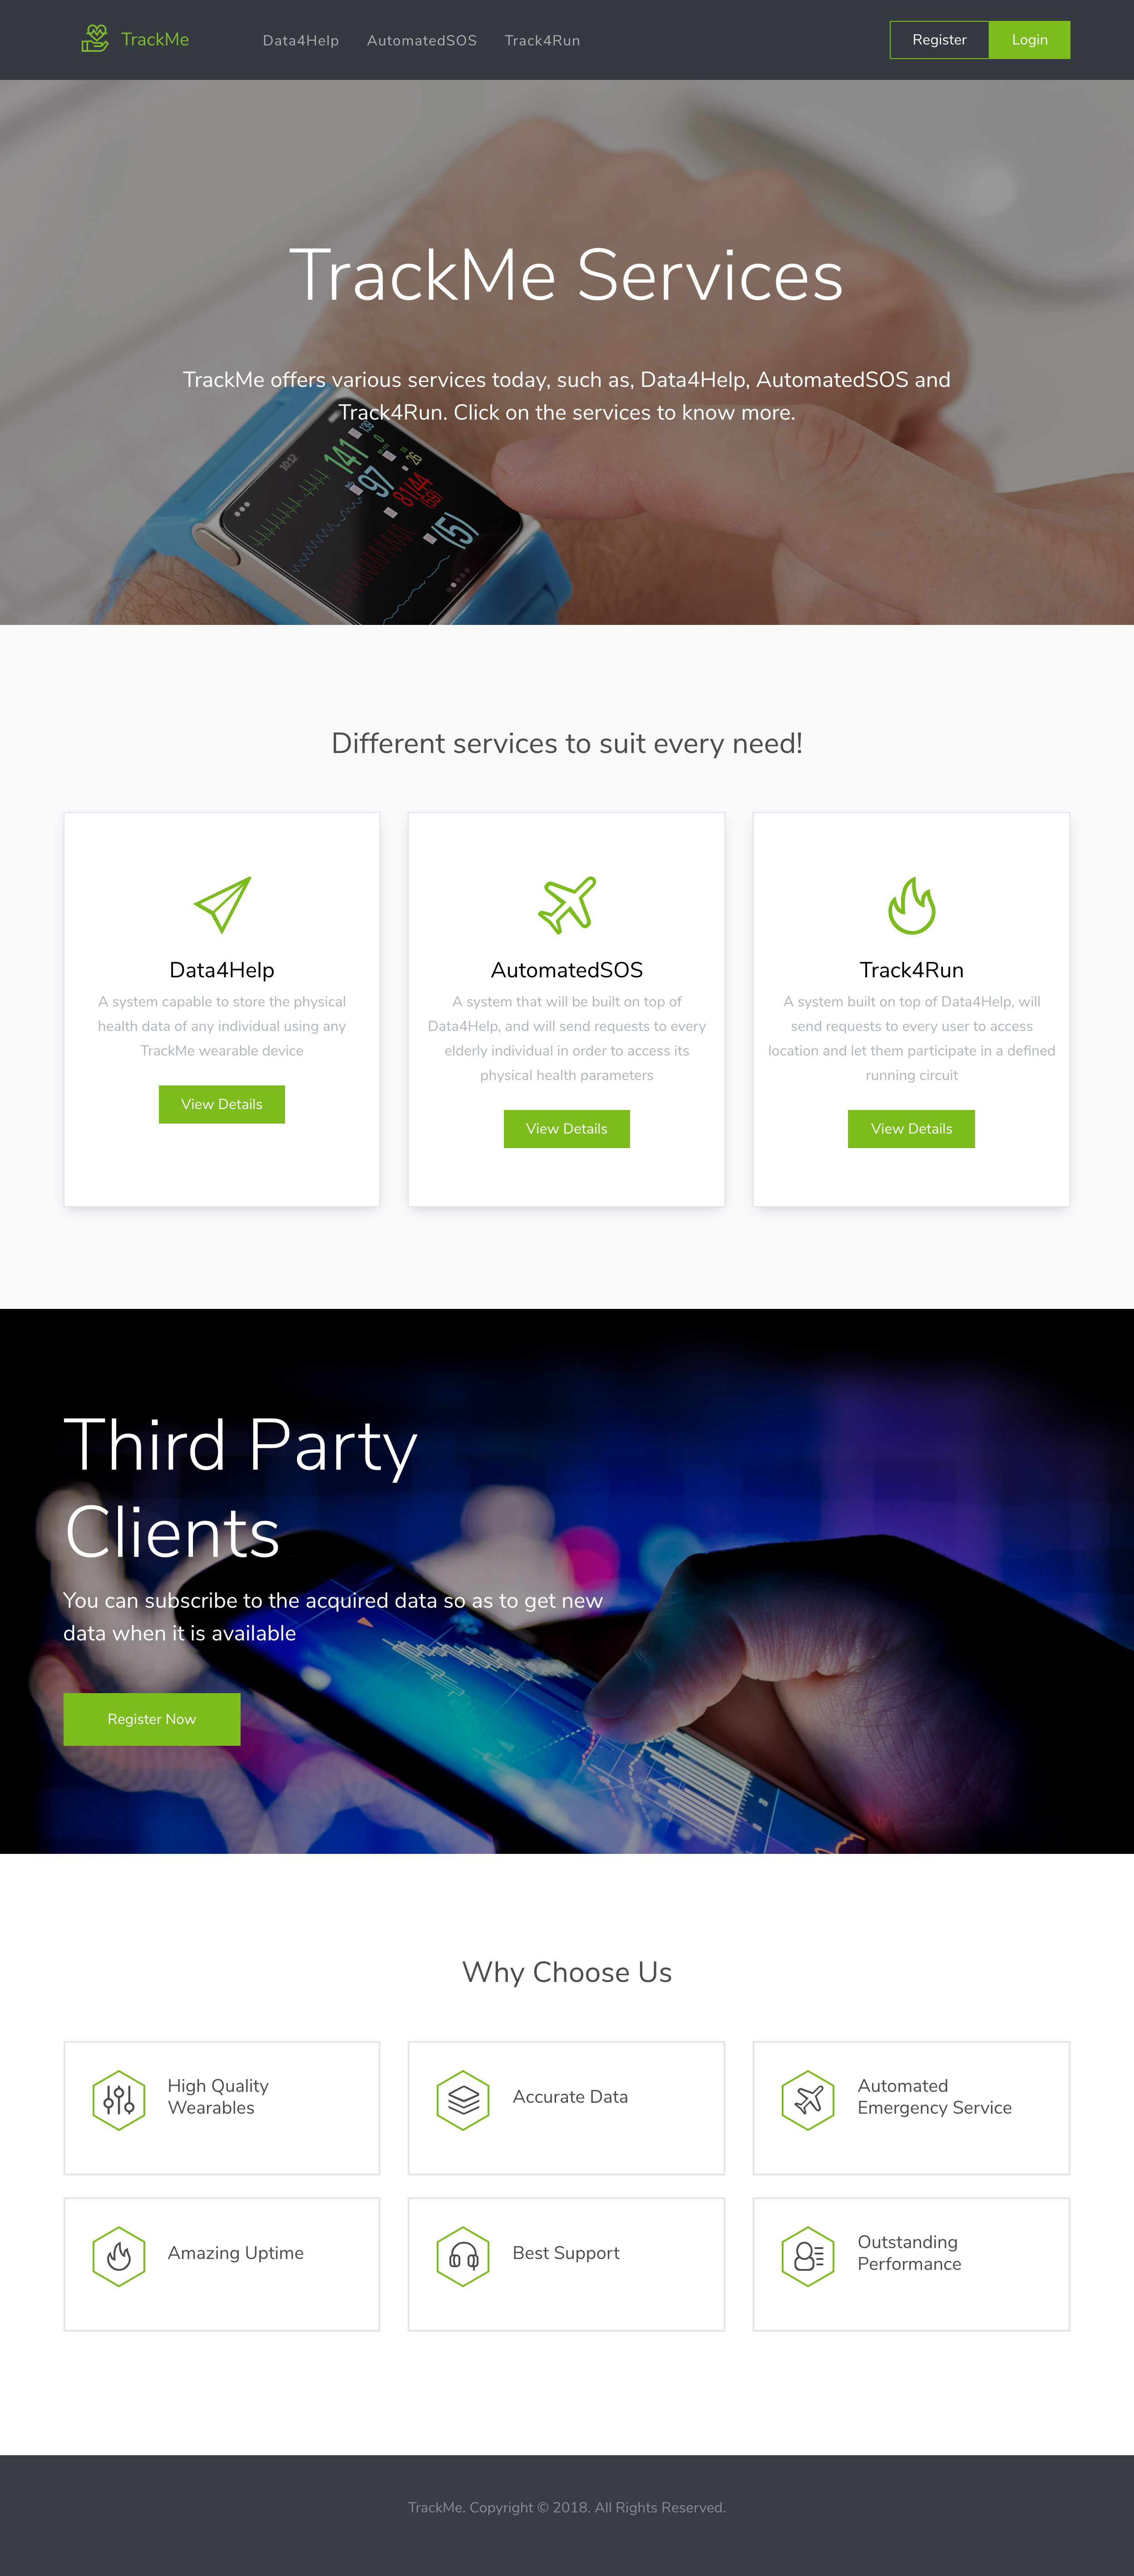
\includegraphics[scale=0.11]{UI/d4h_home.png}
		\caption[UI: TrackMe's Home Page]{TrackMe's Home Page}
		\label{fig:Home_Page}
	\end{figure}
	
	\begin{figure}[H]
		\centering
		\includegraphics[scale=0.13]{UI/d4h.png}

		\caption[UI: Data4Help Information Page]{Data4Help Information Page}
		\label{fig:Data4Help Information Page}
	\end{figure}
	\begin{figure}[H]
		\centering
		\includegraphics[scale=0.13]{UI/asos.png}

		\caption[UI: ASOS Information Page]{ASOS Information Page}
		\label{fig:ASOS Information Page}
	\end{figure}
	
	In the Figure \ref{fig:Login}, can be seen the web page through which users can Login into the system (if already registered).
	
	\begin{figure}[H]
		\centering
		\includegraphics[scale=0.12]{UI/login.png}
		\caption[UI: Login Page]{Login Page}
		\label{fig:Login}
	\end{figure}
	
	 And if not already registered into the system, they can register themselves through the Register web-page (Figure \ref{fig:Registration}). There are separate register forms for the Individual users and for Third Party users.
	 \begin{figure}[H]
		\centering
		\includegraphics[scale=0.13]{UI/register.png}
		\caption[UI: Registration Page]{Registration Page}
		\label{fig:Registration}
	\end{figure}
	
	\begin{figure}[H]
		\centering
		\includegraphics[scale=0.35]{UI/dashboard_individual.png}
		\caption[UI: Individual Dashboard Page]{Individual Dashboard Page}
		\label{fig:Dashboard for individuals}
	\end{figure}

The above figure 3.6 displays the dashboard for individual users, this new page is responsive and a real-time view of the application for the individual user's point of view. the individual user have options to accept or reject any request for data acquisition. As soon as an action is taken upon the request, it gets deleted from the page.

	\begin{figure}[H]
		\centering
		\includegraphics[scale=0.35]{UI/db_thirdparty.png}
		\caption[UI: Third party Dashboard Page]{Third party Dashboard Page}
		\label{fig:Dashboard for individuals}
	\end{figure}
	The above figure 3.7 displays the dashboard for third party users, this new page is responsive and a real-time view of the application for the third party user's point of view. Third parties can  request for  data using the filtering criteria provided by the system such as: specific individual data or in bulk; furthermore, if its specific request then filtering is done by SSN/fiscal code and if its bulk data, then, filtering is done basis upon country, age and blood type.
	
	
	\begin{figure}[H]
		\centering
		\includegraphics[scale=0.35]{UI/db_organizer1.png}
		\caption[UI: Organizers' Dashboard Page]{Organizers' Dashboard Page}
		\label{fig:Dashboard for Organizer}
	\end{figure}
	In the figure 3.8, the organizer can see the number of pending invites for the already configured runs which are still pending to send to the targeted participants; also, organizer's are able to view the number of already configured runs from the past; In addition, they can start configuring a new run by clicking on 'Create new run' button.
	
	\begin{figure}[H]
		\centering
		\includegraphics[scale=0.35]{UI/db_organizer2.png}
		\caption[UI: Organizers' Dashboard Page]{Organizers' Dashboard Page}
		\label{fig:Dashboard for Organizer}
	\end{figure}
	In the figure 3.9, Organizer's are able to define the parameters to define a complete running circuit such as: start and end time, name of the run, date of the run, nodes of the running circuit and here they can select whether to send invitations now or not by clicking the check-box; Thus, by clicking on 'Complete running circuit' button, the configuration gets completed and based on the details above, run is configured.
	
	\begin{figure}[H]
		\centering
		\includegraphics[scale=0.35]{UI/track4run.png}
		\caption[UI: Track4Run Web Page]{Track4Run Web Page}
		\label{fig:Track4Run Web Page}
	\end{figure}
	In the figure 3.10, Spectators are able to view all the available runs in which are currently going on; and by clicking on 'view participants' button, they are redirected to the map-view of the selected run, where they can view the live location of the participant users.
	
	
	\begin{figure}[H]
		\centering
		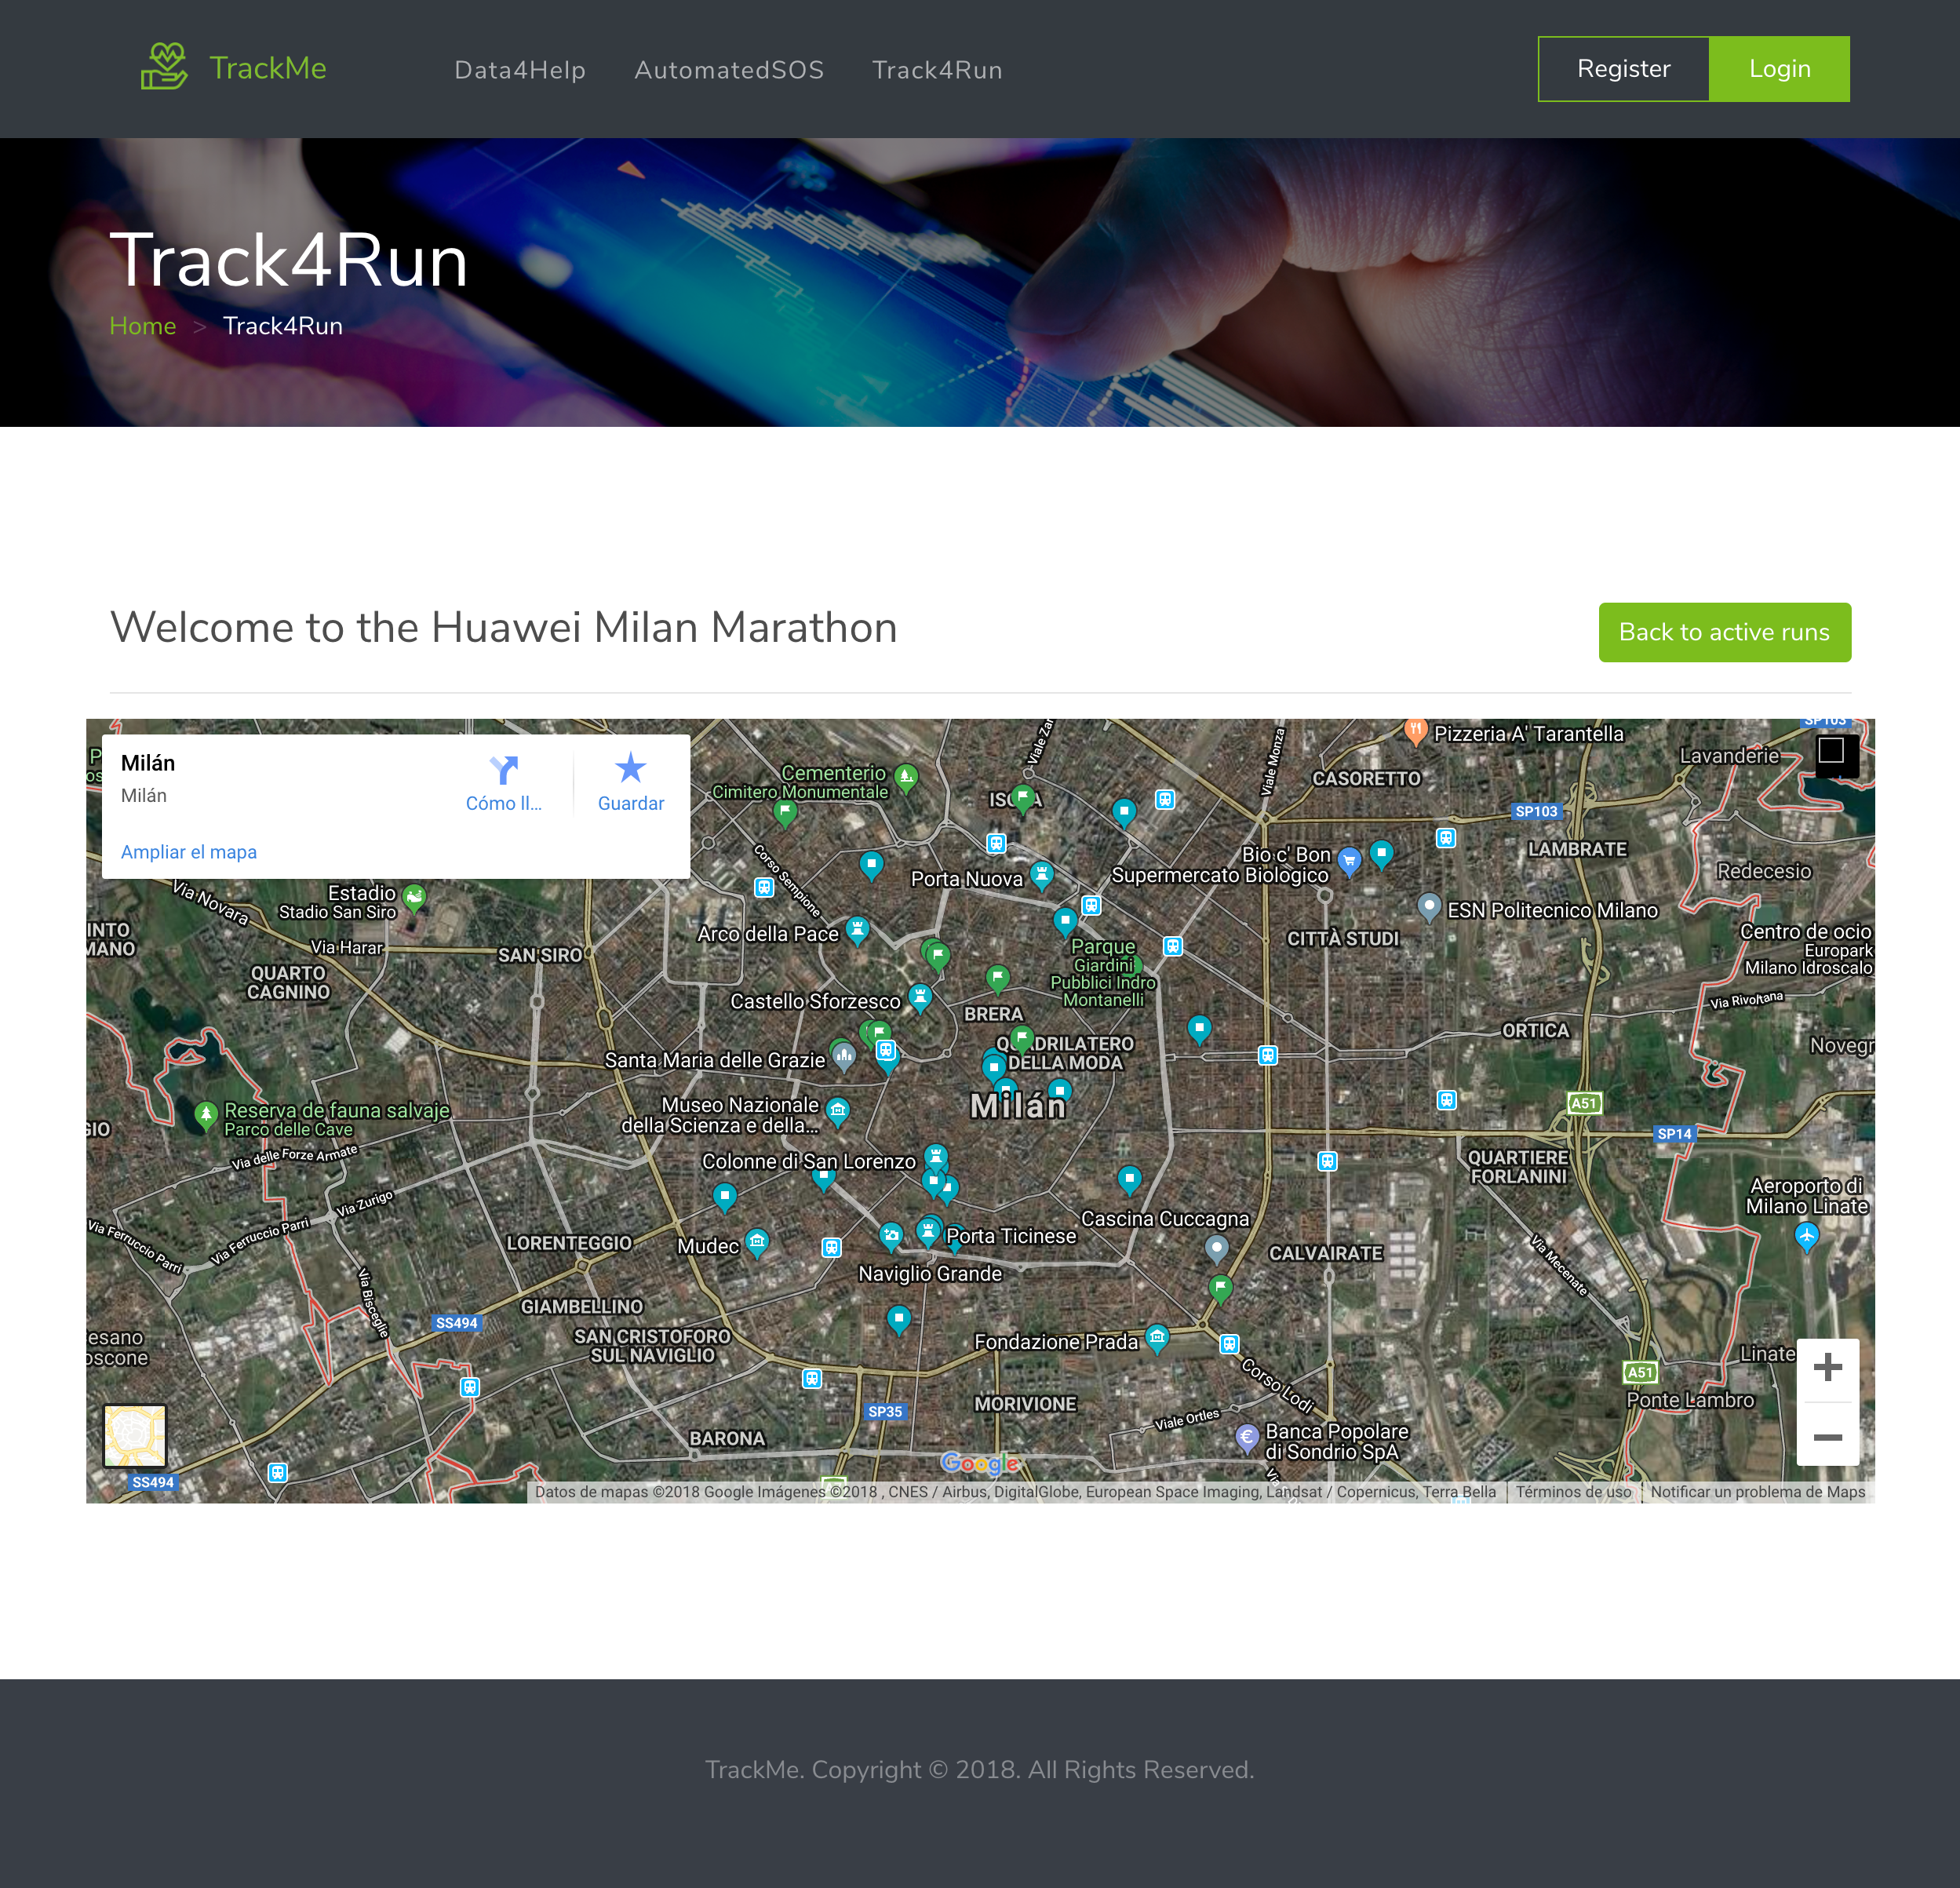
\includegraphics[scale=0.35]{UI/spectators_map.png}
		\caption[UI: Spectators' Map-view Page]{Spectators' Map-view Page}
		\label{fig:Spectators' Map-view Page}
	\end{figure}
	
	In the figure 3.11, Spectators are able to view  the participants' live position during the run and time left for the race to end, because after the end of this time, spectators won't be able to view the map.
	
	
	
	
	\begin{figure}[H]
		\centering
		\includegraphics[scale=0.35]{UI/spectator_invalid.png}
		\caption[UI: Spectators's invalid view]{Spectators's invalid view}
		\label{fig:Spectators's invalid view}
	\end{figure}
	
	In the figure 3.12, Spectators are able to view an error message when the race has been ended. 
	
	\chapter{Requirements traceability}
	In this section is shown how the goals and requirements specified in the RASD are mapped to the design components defined in this document.
	
\begin{itemize}
	\item{\textbf{Data4Help}}
	\begin{enumerate}
		\requirement{1} The system must allow an individual to register a new account \\
		\textbf{D4H::Signup}
		\requirement{2} The system must allow an individual to access to their account \\
		\textbf{D4H::Login}
		\requirement{3} The system must allow an individual to accept or reject their requests of accessing personal data \\
		\textbf{D4H::Request}
		\requirement{4} The system must be able to communicate with TrackMe database in order to obtain the health status and location of an individual \\
		\textbf{D4H::SearchManager}
		\requirement{5} The system must allow a third party company to register a new account \\								\textbf{D4H::Signup}
		\requirement{6} The system must allow a third party company to access to its account 	\\								\textbf{D4H::Login}
		\requirement{7} The system must be able to notify the individual that a third party company wants to access its data \\
		\textbf{D4H::Request}
		\requirement{8} The system must allow a third party company to search for an individual health status and location using his/her SSN \\
		 \textbf{D4H::SearchManager}
		 \requirement{9} The system must allow a third party company to filter data of an anonymized group of individuals by country, age, gender and blood type parameters \\ 
		 \textbf{D4H::SearchManager}
		 \requirement{10} The system must be able to anonymize the data of a group of individuals \\
		 \textbf{D4H::APIManager}
		 \requirement{11} The system must allow a third party company to subscribe to an individual health status and location \\ 
		\textbf{D4H::Subscription}
		\requirement{12} The system must allow a third party company to subscribe to data of an anonymized group of individuals \\
		\textbf{D4H::Subscription}
	\end{enumerate}	
		
	\item{\textbf{AutomatedSOS}}
	\begin{enumerate}
		\requirement{13} The system must be able to send a request for monitoring an individual's data when he/she is older than 60 years old \\
		\textbf{ASOS::DataHandler}
		\requirement{14} The system must be able to monitor, and compare against defined thresholds, the health status of an individual \\
		\textbf{ASOS::DataHandler}
		\requirement{15} The system must be able to contact the health-care service associated to an individual \\
		\textbf{ASOS::HealthCareConnector}
	\end{enumerate}
	
	\item{\textbf{Track4Run}}
	\begin{enumerate}
		\requirement{16} The system must allow a participant to register a new account \\
		\textbf{T4R::Signup}
		\requirement{17} The system must allow a participant to access to their account \\
		\textbf{T4R::Login}
		\requirement{18} The system must allow an organizer to register a new account \\
		\textbf{T4R::Signup}
		\requirement{19} The system must allow an organizer to access to their account \\
		\textbf{T4R::Login}
		\requirement{20} The system must allow an organizer to create a race event \\ 
		\textbf{T4R::Event}
		\requirement{21} The system must allow an organizer to define the running circuit of a race event \\
		\textbf{T4R::Event}
		\requirement{22} The system must allow an organizer to send invitations to participants to enroll in a race event \\
		\textbf{T4R::Notification}
		\requirement{23} The system must allow a participant to accept or reject an invitation to a race \\
		\textbf{T4R::Notification, T4R::Request}
		\requirement{24} The system must allow any spectator of a run to view in a map the participants' location \\ 
		\textbf{T4R::DataHandler}
		\requirement{25} The system must allow a spectator to click on a participant location in order to view his/her health status \\
		\textbf{T4R::DataHandler}
	\end{enumerate}
\end{itemize}

	\chapter{Implementation, integration and test plan}
	\section{Requirements of implementation and testing}
In order to start implementation process of the project, RASD and DD must be finished and available for all the teams of the project, so they will be informed about requirements and adopted design choices. A good analysis of each document is also required to be sure that implemented system will be secure and reliable.\\

\textbf{Development Tools} The Java programming language will be used to develop our system because it suits very well for communication among different platforms and devices. In addition, Java Enterprise Edition will be used to deploy our business functionalities and to build a reliable and powerful web tier to let users communicate with main server using a standard web browser or a Java application. Java Enterprise Edition offers also an enhanced version of JMS services useful for communication between client and server. Spark Framework will be used as it is built for productivity. Spark Framework is a simple and expressive Java/Kotlin web framework DSL built for rapid development. \\

\textbf{Testing Tools} In order to achieve all the testing purposes we will use different testing tools:
\begin{itemize}
\item{} For unit testing of each component we will use \textit{JUnit} framework. It’s a good framework offered by Oracle itself so it’s well test and supported. It can test each functionality of component into an isolated environment. It can be used also to test some little interaction between components.
\item{}\textit{Mockito} tool will be used as it is a No expect-run-verify technique. Mockito is a mocking framework that tastes really good. It lets you write beautiful tests with a clean and simple API. Mockito doesn’t give you hangover because the tests are very readable and they produce clean verification errors.
\item{} \textit{Arquillian} tools may be used during integration testing: it offers different features that tests very well Java Enterprise components and containers. It also provides features for debugging servers functionalities.
\item{} \textit{Grinder} software may be used to make load tests onWeb Server.
\item{} \textit{HammerDB} may be used to test functionalities and performance of Database server.
\end{itemize}


\section{Implementation Strategy}
Implementation process will follow the bottom-up strategy: we plan to implement first single component isolated. Once at least 60\% of a component will be developed, its unit testing phase can start.\\
Using \textit{Drivers} for tests allows different developer teams to complete its own work. Using this method we can be sure that component will be more reliable, so it will be more easy to reuse them into different part of the system.\\

The implementation of the \textit{TrackMe} system will be done module by module and component by component. The order in which it is carried out depends on a number of factors like the complexity of the modules and services, the dependence of other modules on the component being implemented and to the system as a whole, and it should also take into account the possibility of discovering flaws with the proposed design. The later should be dealt in a way that, if such an unfortunate event does	happen, the flaws should be found and corrected as soon as possible, to limit the cost of the change of design. Identify here the order in which system plan to implement the subcomponents of your system and the order in which system plan to integrate such subcomponents and test the integration.\\

\subsection{Implementation order}
Due to modularity of system components and to the adopted strategy there are no constraints on implementation order of components. But due to some critical aspects of a few components we want to prioritize implementation of those components.
The most critical components of the system that could take more than others to be implemented may be:

\begin{enumerate}
\item{} Data4HelpWebService, Track4RunWebService
\item{} LoginService and SignupService
\item{} SearchManager, AuthenticationManager, DBManager, DataHandler
\item{} RequestService, SubscriptionService, NotificationService
\item{} HealthCareService, HealthCareConnector, AutomatedSOSDB
\item{} UserService, TokenDB, Track4RunDB
\end{enumerate}
(note that by specifying the names of interfaces of components, we are also considering the concrete implementations, in whichever number they exist)\\

The Data4HelpWebService is proposed to be the first component that is implemented because all parts of the application server will be using some element of it and its role in allowing some service to communicate with the DBMS in the DBManager component is crucial to the whole application. The component releasing process should follow the integration order that will be described into the next section.

\section{Integration and Testing}
\subsection{Entry criteria} 
The integration of components and its testing should start as soon as possible, but before they can commence, some conditions must be met. First of all, the external services and their APIs that are going to be used in the application should be available and ready. This applies to the already mentioned services, to the DBMS and the server on which it will be running on. \\

Next, the modules which are being integrated should have at least the operations concerning one another created, if not completed completely. The operations that have been developed should pass the unit tests in order to be sure that the components are working fine on their own and that if an integration test fails, the problem lies in the in the integration itself.\\

\subsection{Integration test strategy}  
The main goal of integration process is to avoid as much
errors as possible at each step of the process, so the system will incrementally integrate components as soon as they are completely developed and released.\\

\textit{Bottom-up} design will be adopted for most of the integration process: at the beginning only components that have less bindings to other components or which can work without other component will be integrated. In this way we can obtain feedbacks
about system functionalities as soon as components are released and in addition we can parallelize integration of different subsections of the system.\\

For the most critical components or for more complex system parts we will use instead \textit{Critical Modules strategy}: components that fit very well for \textit{Critical Modules} strategy are those in Data4Help subsystem, because the AutomatedSOS and Track4Run will use the Data4Help system and are the most frequent interaction performed into our system. For this reason \textit{Bottom-Up} strategy will be applied only once Data4Help subsystem will be fully integrated using \textit{Critical Modules}.

\subsection{Integration order}
In this section, the list and order of every integration that is performed is shown. As already stated, the integration will be performed from the bottom-up. \\

It should be noted that there will be no explicit integration of the Data4HelpWebService, Track4RunWebService with any of the other components. This is because the nature of the component, the extent of the usage and dependency of other components on it and the implementation plan, that clearly states that the Data4HelpWebService will be the first part that is implemented, mean that the integration itself is already being done during the implementation phase of the depending components and its correctness will inherently be tested by the unit tests of each component.
\begin{enumerate}
\item{} As written in the introduction, at the beginning we will integrate the \textit{Data4Help} subsystem, composed by these components:
\begin{itemize}
\item{} Data4HelpWebSite
\item{} LoginService and SignupService
\item{} RequestService and NotificationService
\item{} SubscriptionService
\end{itemize}

Integration tests will check cases like addition of new user to database, accessing the system with correct credentials, the consistency of making request, the reachability of all notifications to accept/reject request in the dashboard, the modification of subscription chosen by the user (if he wants any).

\item{} Then we could start to implement part of the \textit{AutomatedSOS} subsystem:
\begin{itemize}
\item{} HealthCareService (\textit{External component})
\item{} HealthCareConnector 
\item{} AutomatedSOSDB
\item{} ThresholdCollection, UserCollection, HealthCareCollection
\end{itemize}
This integration step will check the communication of the Data4Help system with external sources HealthCareService when the vital signs are out of the normal range or the ThresholdCollection.

\item{} Then we could start to implement part of the \textit{Track4Run} subsystem:
\begin{itemize}
\item{} Track4RunWebService
\item{} Track4RunDB 
\item{} RunCollection
\item{} TokenService, OrganizerCollection and ParticipantCollection
\end{itemize}
This integration step will check the communication of the Data4Help system with Track4RunWebService and when RunCollection is modified, check the integration with the existing requestService and notificationService of Data4HelpWebService.

\item{} After that, other components can be joined together into small subsystems to test their interactions:
\begin{itemize}
\item{} \textit{AuthenticationManager} and \textit{LoginService} : their interactions must not brake the consistency of Account information and they have to check only authorized users can access information
\item{} \textit{SearchManager, RequestService} and \textit{SubscriptionService} : system will check consistency between search into a request and subscription of the same user
\item{} \textit{DataHandler, DBManager} and \textit{HealthCareConnector} : system will continuously check latest data and verify with the ThresholdCollection, if varies, notifies HealthCareService through HealthCareConnector of the same user
\item{} \textit{RunCollection} and \textit{ParticipantCollection} : system will check consistency between run created and allows users participated in the same run
\end{itemize}

\item{} After that we can start to integrate user interactions:
\begin{itemize}
\item{} \textit{UserInterface} and \textit{RequestService} : tests sending request for specific or anonymized search through different user interfaces
\item{} \textit{UserInterface} and \textit{NotificationService} : tests will check asynchronous communication between user and server for the dispatch of event messages
\item{} \textit{UserInterface} and \textit{RunCollection} : tests will check asynchronous communication between user and runs available for the live view on the map of participants
\item{} \textit{UserInterface} and \textit{HealthCareService} External Resource : will tests the communication
with external services of User Interface and Health-Care Service
and the synchronization of Data with threshold values when user's data is out of range, notifies using external alarm interfaces
\end{itemize}
\end{enumerate}
	
	\chapter{Effort spent}
	\begin{table}[h]
		\centering
		\begin{tabular}{l c}
			\hline\hline
			\multicolumn{2}{c}{\textbf{Team Work}} \\
			\hline
			\textbf{Task} & \textbf{Hours} \\ [0.5ex]
			\hline
			Planning Architecture & 3  \\
			Choosing Pattern & 2 \\
			Algorithm Decisions & 8 \\
			Checking document  & 4  \\
			\hline
			\textbf{Total} & 17  \\
			\hline
		\end{tabular}
		\caption{Time spent by all team members}
		\label{fig:Time spent by all team members}
	\end{table}
	
	\begin{table}[h]
		\centering
		\begin{tabular}{l c l c l c}
			\hline\hline
			\multicolumn{6}{c}{\textbf{Individual Work}} \\
			\hline
			\multicolumn{2}{c |}{\textbf{Diego Avila}}  &
			\multicolumn{2}{c |}{\textbf{Laura Schiatti}} &
			\multicolumn{2}{c}{\textbf{Sukhpreet Kaur}}  \\
			\hline
			\textbf{Task} & \textbf{Hours}
			& \textbf{Task} & \textbf{Hours}
			& \textbf{Task} & \textbf{Hours} \\ [0.5ex]
			\hline
			X &  X
			& Layout & X
			& X & X  \\
			\hline
			\textbf{Total} & X
			& \textbf{Total} & X
			& \textbf{Total} & X  \\
			\hline
		\end{tabular}
		\caption{Time spent by each team member}
		\label{fig:Time spent by each team member}
	\end{table}
	
	\chapter{References}
	\begin{itemize}
		\item Requirement Analysis and Specification Document: AA 2017-2018.pdf”. Version 1.0 - 26.10.2017
		\item Henriksen, A., Haugen Mikalsen, M., Woldaregay, A. Z., Muzny, M., Hartvigsen, G., Hopstock, L. A., Grimsgaard, S. (2018)
		\\Using Fitness Trackers and Smartwatches to Measure Physical Activity in Research: Analysis of Consumer Wrist-Worn Wearables. Journal of medical Internet research, 20(3), e110. doi:10.2196/jmir.9157.
		\\Retrieved from: https://www.ncbi.nlm.nih.gov/pmc/articles/PMC5887043/
		\item IEEE. (1993). IEEE Recommended Practice for Software Requirements Specifications (IEEE 830-1993).
		\\Retrieved from https://standards.ieee.org/standard/830-1993.html
		\item Sloane, A. M. (2009). Software Abstractions: Logic, Language, and Analysis by Jackson Daniel, The MIT Press, 2006, 366pp, ISBN 978-0262101141.
	\end{itemize}
	
\end{document}